% Computer Vision Final Project Template
% based on CVPR 2022 template, which is further based on CVPR template provided by Ming-Ming Cheng (https://github.com/MCG-NKU/CVPR_Template)
% modified and extended by Stefan Roth (stefan.roth@NOSPAMtu-darmstadt.de)

\documentclass[10pt,twocolumn,letterpaper]{article}

%%%%%%%%% PAPER TYPE  - PLEASE UPDATE FOR FINAL VERSION
\usepackage{cvpr}              % To produce the CAMERA-READY version
\usepackage{ctex}

% Include other packages here, before hyperref.
\usepackage{graphicx}
\usepackage{amsmath}
\usepackage{amssymb}
\usepackage{booktabs}
\usepackage{enumitem}


% It is strongly recommended to use hyperref, especially for the review version.
% hyperref with option pagebackref eases the reviewers' job.
% Please disable hyperref *only* if you encounter grave issues, e.g. with the
% file validation for the camera-ready version.
%
% If you comment hyperref and then uncomment it, you should delete
% ReviewTempalte.aux before re-running LaTeX.
% (Or just hit 'q' on the first LaTeX run, let it finish, and you
%  should be clear).
\usepackage[pagebackref,breaklinks,colorlinks]{hyperref}


% Support for easy cross-referencing
\usepackage[capitalize]{cleveref}
\crefname{section}{Sec.}{Secs.}
\Crefname{section}{Section}{Sections}
\Crefname{table}{Table}{Tables}
\crefname{table}{Tab.}{Tabs.}


%%%%%%%%% PAPER ID  - PLEASE UPDATE
\def\cvprPaperID{*****} % *** Enter the CVPR Paper ID here
\def\confName{CVPR}
\def\confYear{2022}


\begin{document}

%%%%%%%%% TITLE - PLEASE UPDATE
\title{张量分解在神经辐射场渲染中的应用}

\author{刘佳润\\
    22221290\\
    计算机科学与技术学院\\
    {\tt\small jiarunliu@zju.edu.cn}
}
\maketitle

%%%%%%%%% ABSTRACT
\begin{abstract}
  张量分解(Tensor Decomposition)是一种在标量分解、向量分解以及矩阵分解算法的基础上进行泛化的经典算法,
  其在降维处理、稀疏性分析以及隐性关系挖掘中具有重要的作用。近年来随着三维计算机视觉的高速发展,一种基于隐式
  表达的三维场景新视角渲染的方法——神经辐射场(Neural Radiance Field, NeRF)在该领域取得了极大的成功。
  然而大多数的NeRF方法在训练速度、神经网络复杂程度等方面存在许多缺陷。本文结合近两年来前沿工作,分析张量分解
  在NeRF中的应用与改进,分析其优越性并进行推演梳理和总结。
\end{abstract}

%%%%%%%%% BODY TEXT
\section{引言}
\label{sec:intro}
在计算机科学中,张量是对矩阵这一概念的扩充,作为一种数据容器,在诸如计算机图形学、计算机视觉、并行计算、深度学习等领域有非常重要的意义。相应地,张量分解技术在其中也具有非常重要的地位。与矩阵分解类似,张量分解具有数据降维、稀疏数据分析与填充、隐性关系挖掘的重要作用,尤其是对于稀疏张量,张量分解\cite{kolda2009tensor}是一种常用的分析方法。

在三维计算机视觉领域,一种近年来发展迅速的解决新视角合成问题的方法逐渐被人们所重点关注,即神经辐射场(Neural Radiance Field, NeRF)\cite{mildenhall2021nerf}。NeRF是一种面向三维隐式空间建模的基于多层感知机(Multi-Layer Perception, MLP)的深度学习模型。由于MLP的隐式表达,这种方法可以非常简洁的对三维场景进行建模。然而,由于深度学习的网络参数量大、模型结构复杂,导致许多经典NeRF算法难以避免训练、推理速度慢、模型空间大等问题。针对此,许多近期工作在MLP的基础上,加入一些显式的混合表达方式来将一些3D特征存储在显示的数据结构中,从而优化其效果。

将张量分解技巧应用到NeRF问题中,是一种非常优雅的数学方法。由于辐射场和三维空间的特性十分契合高阶张量的表示方法,同时具有很高的稀疏性质,因此利用张量分解,将辐射场分解为若干紧凑度高的成分,可以很好的对辐射场的特征值、表征值等进行建模。近年如TensoRF\cite{chen2022tensorf},CCNeRF\cite{tang2022ccnerf}等工作将张量分解应用到NeRF场景中,获得了很好的提升效果,并证明了这一工作的可扩展性,INS\cite{li2023instant}、StyleRF\cite{liu2023stylerf}等工作在此基础上的扩展与优化也验证了该方法的高效。

本文结合以上提到的若干工作进行脉络梳理与方法总结,并探索使用张量表达以及张量分解在辐射场视觉问题上的原理和可优化原因。本文第\ref{sec:related_work}节将讨论张量分解的原始形式数学原理以及NeRF的基本原理。本文第\ref{sec:td}节将具体讨论三种张量分解方法以及其在NeRF中的结合成果,其中\ref{sec:cp}、\ref{sec:vm}将针对TensoRF\cite{chen2022tensorf}的方法进行原理剖析,\ref{sec:hy}将针对CCNeRF\cite{tang2022ccnerf}的方法进行原理剖析,并指出其与前两节的联系。本文第\ref{sec:analysis}节将具体分析以上方法在NeRF中的应用,以及通过实验结果进行分析并探讨该方法的优越性。本文第\ref{sec:conclusion}节将做出总结,并讨论未来可扩展研究方向。
%-------------------------------------------------------------------------
\section{背景知识}
\label{sec:related_work}

\subsection{低阶张量分解}
矩阵是一种典型的低阶(二阶)张量,因此可以从矩阵分解中理解张量分解的意义。常见的矩阵分解方式很多,本文应用的分解算法思路主要基于奇异值分解(Single Value Decomposition, SVD)\cite{hoecker1996svd}。

SVD分解的基本思想是将矩阵分解为两个因子矩阵和一个奇异值对角矩阵。对于任意一个矩阵$\bold M\in\mathbb R^{m\times n}$,可以将其写作如下形式:
\begin{equation}
  \bold M_{m\times n} = \bold U_{m\times m} \bold \Sigma_{m\times n} \bold V_{n\times n}^\top
\end{equation}
\label{eq:1}
其中,$\bold U, \bold V^\top$是酉矩阵,$\bold \Sigma$主对角线上的元素即为原矩阵$\bold M$的奇异值。这样的分解方式可以寻找数据分布的主要维度,将原始的高维数据映射到低维子空间中,从而实现数据降维,或是寻找到原始数据的主要特征。

\subsection{神经辐射场(NeRF)}
给定一组图像集,NeRF旨在渲染新视角下的照相级别的逼真图像。NeRF的基本思想是使用一个5自由度参数(目标点位置$\bold x\in\mathbb R^3$,观测方向向量$\bold d\in\mathbb R^2$)来表示任意一张新视角合成图像,并利用体渲染方法来提高渲染质量。

NeRF利用MLP对场景进行软编码,通过上述输入分别学习体密度(不透明度场)$\sigma$以及依赖于视图的表面纹理的辐射场(颜色)$\bold c$。通过体渲染方式,根据训练出的不透明度场和辐射场以及给定光线和观测方向,通过采样和积分的方法可以得到像素颜色:
\begin{equation}
  \mathbf{C}(\mathbf{r})=\int_{t=0}^{\infty} \sigma(\mathbf{o}+t \mathbf{d}) \cdot \mathbf{c}(\mathbf{o}+t \mathbf{d}, \mathbf{d}) \cdot e^{-\int_{s=0}^{t} \sigma(\mathbf{o}+s \mathbf{d}) d s} d t
\end{equation}
\label{eq:2}
上述过程如图\ref{fig:nerf}所示。
\begin{figure}[b]
  \centering
  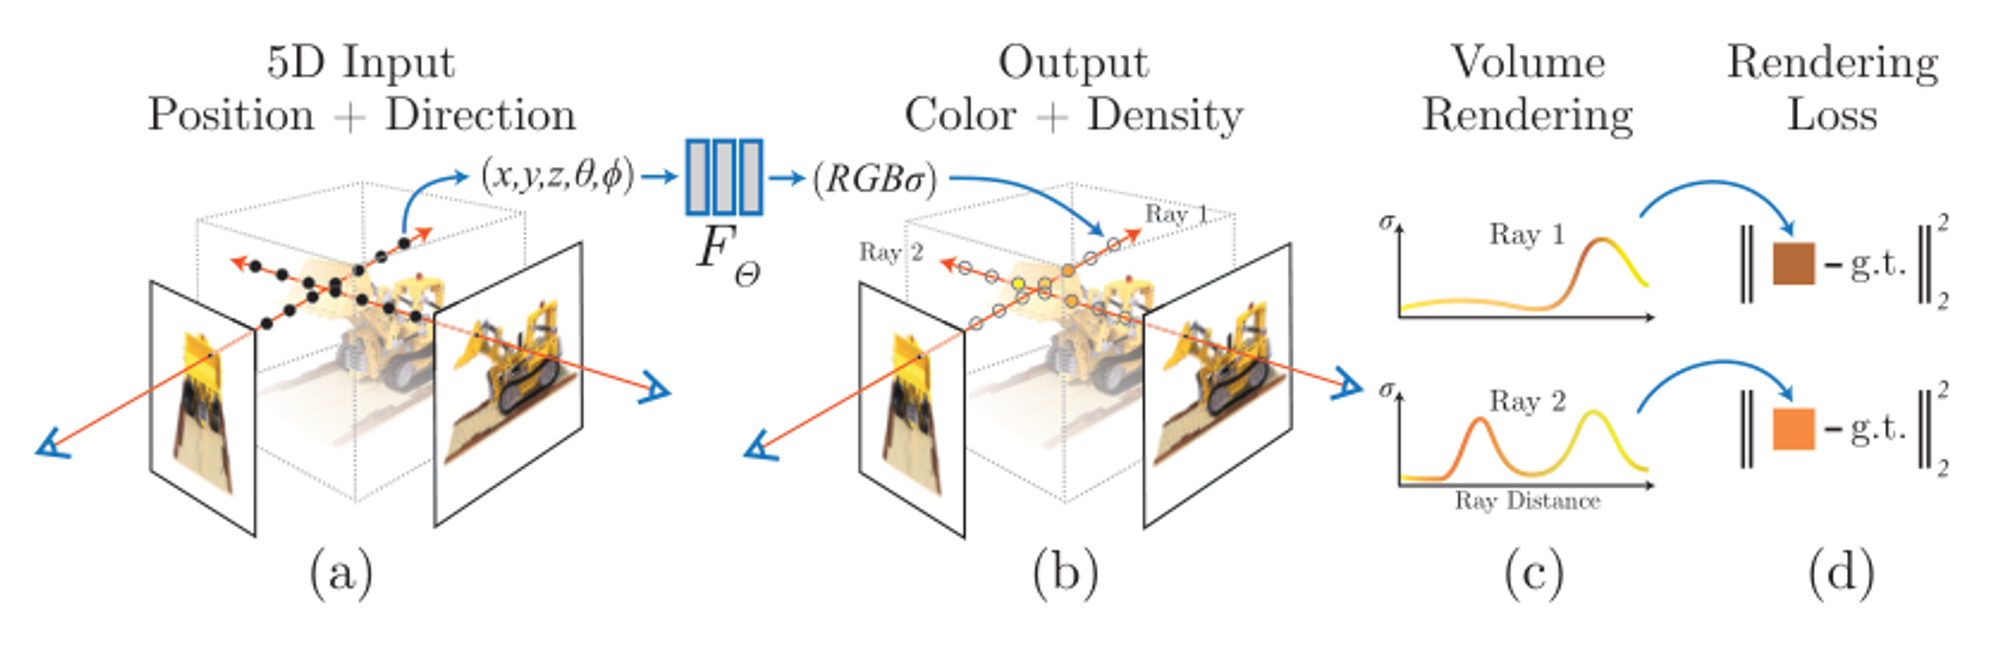
\includegraphics[width=1.0\linewidth]{fig/nerf.png}
  \caption{NeRF方法原理示意图}
  \label{fig:nerf}
\end{figure}

NeRF中需要学习的是对$\sigma$以及$\bold c$的预测模型。实践中的经典损失函数是真实颜色与预测颜色的平方误差损失,即只需要通过拍摄到的图像就可以进行监督与训练。

%-------------------------------------------------------------------------
\section{张量分解方法}
\label{sec:td}

\begin{figure}
  \centering
  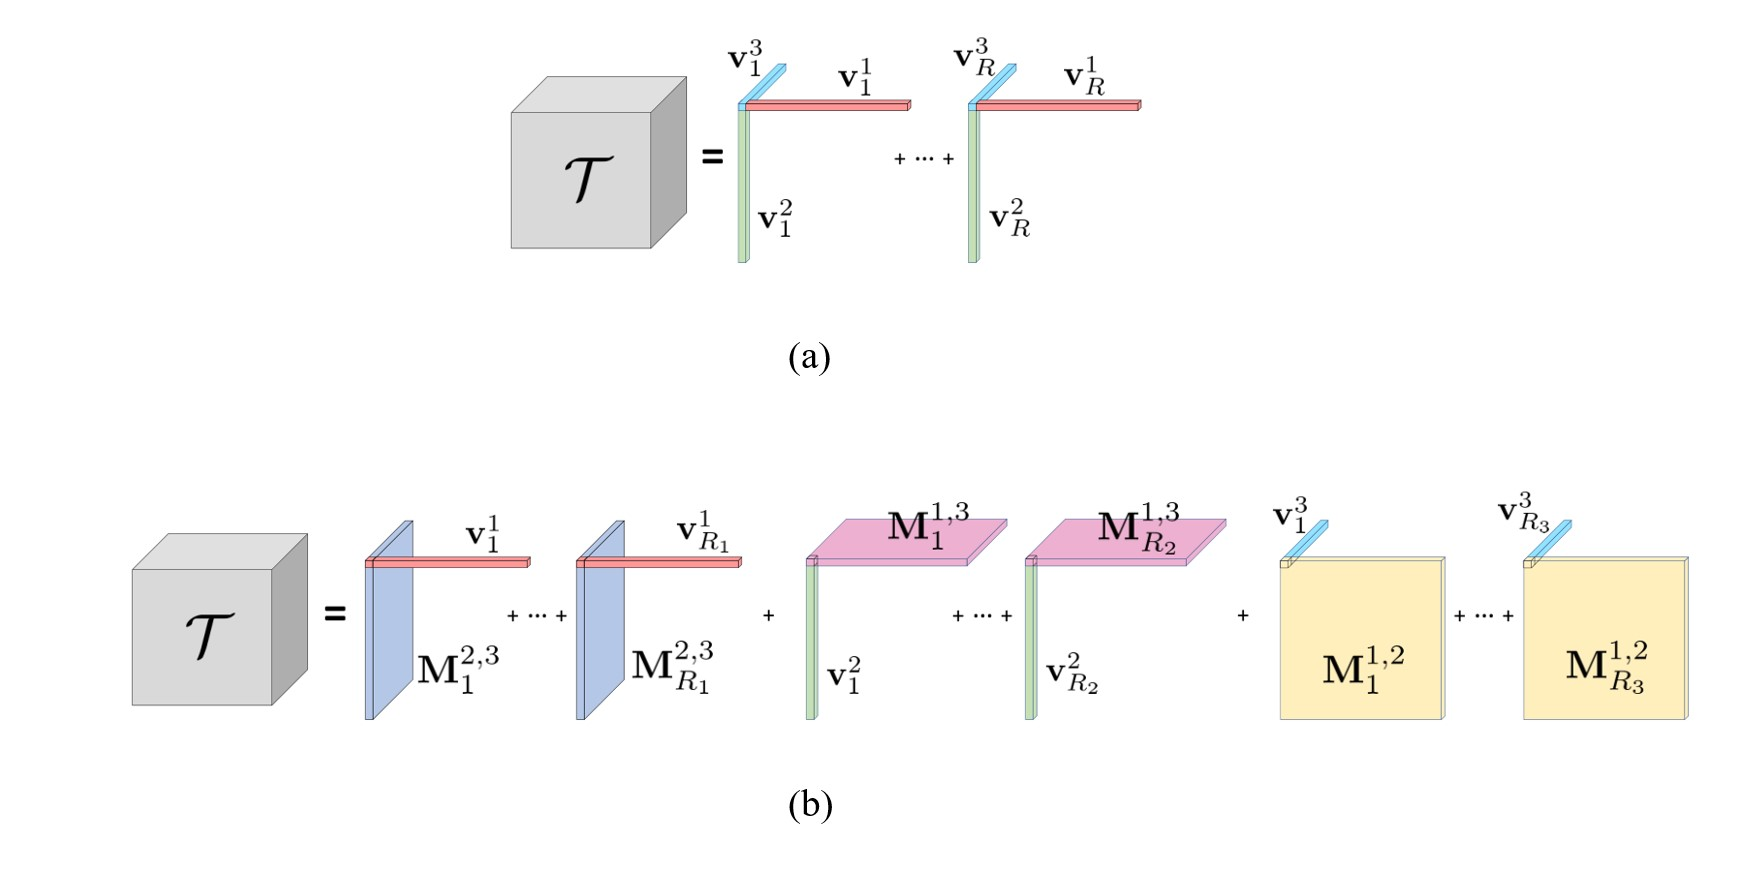
\includegraphics[width=1.0\linewidth]{fig/CPVM.jpg}
  \caption{两种经典张量分解方式。(a)CP分解,(b)VM分解}
  \label{fig:cpvm}
\end{figure}

\subsection{CP分解}
\label{sec:cp}
在对SVD分解进行高阶扩张的过程中,一种推演方法被称为CP分解(Canonical Polyadic Decomposition)\cite{harshman1970cpd}。SVD分解将矩阵分解为奇异值矩阵和正交矩阵因子之积,而CP分解则是将张量分解为若干秩一张量的和,其中每一个秩一张量可以表示为若干向量的外积。如图\ref{fig:cpvm}(a)所示,对于一个三维张量$\mathcal T\in\mathbb R^{I\times J\times K}$,可以对其进行$R$个成分的CP分解:
\begin{equation}
  \mathcal{T}=\sum_{r=1}^{R} \mathbf{v}_{r}^{1} \circ \mathbf{v}_{r}^{2} \circ \mathbf{v}_{r}^{3}
\end{equation}
\label{eq:3}
其中$\circ$代表矩阵外积,每一个$\bold v^1_r\circ\bold v^2_r\circ\bold v^3_r$,对应一个秩一张量成分,其中$\bold v^1_r\in\mathbb R^I,\bold v^2_r\in\mathbb R^J,\bold v^3_r\in\mathbb R^K$,代表第$r$个成分三个分解向量。

CP分解的计算可以通过交替最小二乘法(ALS)实现。CP分解将张量分解为多个向量,表示多个紧致的秩一分量。这个过程是一个对高阶张量进行简化和重点成分提取的过程,因此常用于神经网络的压缩,同时也可能作为辐射场场景的建模。

\subsection{VM分解}
\label{sec:vm}
CP分解的方式保证了多个张量分量的低秩性与紧凑型,然而由于紧凑性太高,CP分解可能需要许多组件来对复杂场景进行建模,导致辐射场重建的计算成本很高。在此基础上TensoRF\cite{chen2022tensorf}工作进行了扩展,引入了更加灵活的VM分解(Vector-Matrix Decomposition)。

如图\ref{fig:cpvm}(b)所示,与利用纯向量因子的CP分解不同,VM分解将张量分解为多个向量和矩阵:
\begin{equation}
  \mathcal{T}=\sum_{r=1}^{R_{1}} \mathbf{v}_{r}^{1} \circ \mathbf{M}_{r}^{2,3}+\sum_{r=1}^{R_{2}} \mathbf{v}_{r}^{2} \circ \mathbf{M}_{r}^{1,3}+\sum_{r=1}^{R_{3}} \mathbf{v}_{r}^{3} \circ \mathbf{M}_{r}^{1,2}
\end{equation}
\label{eq:4}
具体而言,该方法不是使用单独的向量,而是将每两种模式组合起来,并用矩阵表示它们,从而允许用较少的分量对每个模式进行充分的参数化。对每个分解成分,以第一项为例,第一个模式$\bold v^1_r$一定是秩为1的,而第二模式和第三模式的秩可以随意,取决于组合的矩阵$\bold M^{2,3}_r$的秩。这样就降低了CP分解的紧凑性要求,同时可以指定分解的成分数量$R_1,R_2,R_3$,根据每个模的复杂性来另外设置。

注意到在CP分解中,每个分量张量都比一个分量有更多的参数。虽然VM分解会导致较低的紧凑性,但VM分量张量可以表达比CP分量更复杂的高维数据,从而在对同一复杂函数建模时减少所需的分量数量。另一方面,与体素或网格的表示方法相比,VM分解仍然具有非常高的紧凑性,但是能够将计算的复杂性从$O(N^3)$降低为$O(N^2)$。


\subsection{HY分解}
\label{sec:hy}
VM分解虽然放宽了CP分解的约束,同时发明了一种符合三维场景以及特征通道结合的建模方式,但是仍然具有一定的缺陷。首先,VM分解中使用MLP进行场景建模会扰动秩分解的结果并使得其无法进行压缩与组合。其次,VM分解虽然有效结合了秩一向量和矩阵的组合,但是每一个成分内的向量和矩阵的结合过于耦合,导致整体建模的灵活程度收到一定影响。因此,CCNeRF\cite{tang2022ccnerf}中提出的HY分解(Hybrid Variant Decomposition)本质上是对VM分解的进一步解耦,将向量因子和矩阵因子分别分解。

具体而言,在CP分解这种向量分子分解的方法基础上,可以进行扩展。首先,从分解成分上,可以将分解成分由低秩紧密的向量放松为向量组合的矩阵,可以将式\ref{eq:3}修改为:
\begin{equation}
  \mathcal{T}=\sum_{r=1}^{R_{2}} \mathbf{M}_{r}^{1,2} \circ \mathbf{M}_{r}^{1,3} \circ \mathbf{M}_{r}^{2,3}
\end{equation}
\label{eq:5}
其中的$\mathbf M$代表沿着三个平面的因子矩阵。直观地,这种变式指的是首先沿着每个轴对原始3D空间进行切片和平铺,然后在$\mathbb R^{XY\times XZ\times YZ}$ 上进行CP分解。将这种变式被称为TP分解(Triple Plane Decomposition)。

此外,注意到对于每个单独的秩,基本的基于向量或矩阵的分解可以独立选择。因此,提出了一种将上述CP和TP分解相结合的混合变体分解(Hybrid Variant,HY)。如图\ref{fig:hy}所示,HY分解实质上是对CP分解和TP分解的加权组合,同时可以灵活的设置两种成分的分解个数,记为$R=R_{\text{vec}}+R_{\text{mat}}$。HY分解的公式如下:
\begin{equation}
  \mathcal{T}=\alpha\sum_{r=1}^{R_{vec}} \mathbf{v}_{r}^{1} \circ \mathbf{v}_{r}^{2} \circ \mathbf{v}_{r}^{3}+\beta\sum_{r=1}^{R_{2}} \mathbf{M}_{r}^{1,2} \circ \mathbf{M}_{r}^{1,3} \circ \mathbf{M}_{r}^{2,3}
\end{equation}
\label{eq:6}

\begin{figure}[h]
  \centering
  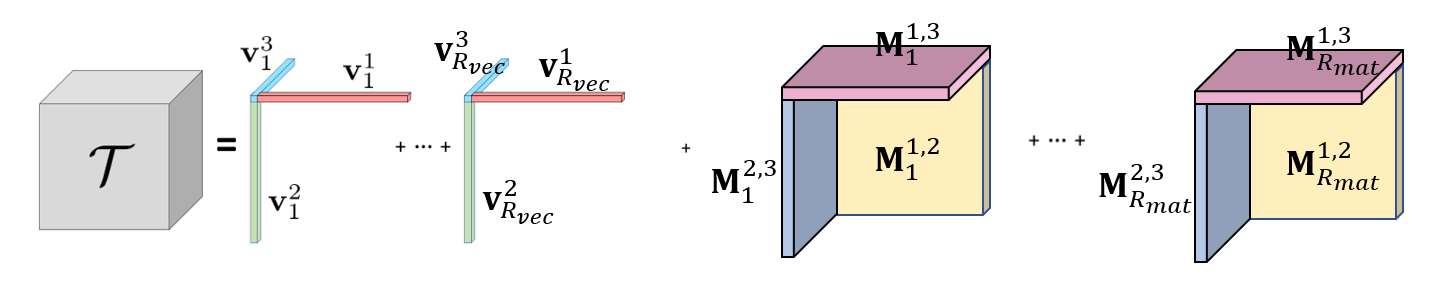
\includegraphics[width=1.0\linewidth]{fig/hy.png}
  \caption{HY分解图示}
  \label{fig:hy}
\end{figure}


\section{辐射场应用与原理分析}
\label{sec:analysis}

\subsection{张量辐射场}
显然,VM分解是对于CP分解的一种泛化表示。在NeRF的建模中,可以通过利用具有每体素多通道特征的规则3D网格$\mathcal G$来对这样的函数进行建模。通过特征通道可将其拆分为几何网格$\mathcal G_σ$和外观网格$\mathcal G_c$,分别对体积密度和视图相关颜色进行建模。其中,$\mathcal G_c$支持各种类型的外观特征,这取决于预先选择的函数$S$,该函数将外观特征向量和视角方向$d$转换为颜色$c$。函数可以选择小的MLP或者球谐函数。同时,只需要用一个单通道的几何网格$\mathcal G_\sigma$来进行体密度表示,不需要其他任何的转换函数。基于连续网格的辐射场可以表示为:
\begin{equation}
  \sigma, c=\mathcal{G}_{\sigma}(\mathbf{x}), S\left(\mathcal{G}_{c}(\mathbf{x}), d\right)
\end{equation}
\label{eq:7}

具体而言,$\mathcal G_\sigma\in\mathbb R^{I\times J\times K}$,分别代表特征网格沿XYZ轴的分辨率,$\mathcal G_c\in\mathbb R^{I\times J\times K\times\ P }$,其中$P$是外观特征通道的数量。3D的几何张量可以由式\ref{eq:4}进行标准的VM分解,4D的外观张量多了一个模式,用来表示特征通道的维度,通常这个维度要远小于XYZ分辨率,即$P \ll I\approx J\approx K$,因此这个张量的秩会比较低。因此,我们不将该模式与矩阵因子中的其他模式相结合,而是仅使用向量,用$\bold b_r$表示,用于因子分解中的该模式。两个张量的分解公式分别如下:
\begin{equation}
  \begin{aligned}\mathcal{G}_{\sigma}&=\sum_{r=1}^{R_{\sigma}} \mathbf{v}_{\sigma, r}^{X} \circ \mathbf{M}_{\sigma, r}^{Y Z}+\mathbf{v}_{\sigma, r}^{Y} \circ \mathbf{M}_{\sigma, r}^{X Z}+\mathbf{v}_{\sigma, r}^{Z} \circ \mathbf{M}_{\sigma, r}^{X Y}\\&=\sum_{r=1}^{R_{\sigma}} \sum_{m \in X Y Z} \mathcal{A}_{\sigma, r}^{m}\end{aligned}
\end{equation}
\label{eq:8}
\begin{equation}
  \begin{aligned}\mathcal{G}_{c} & =\sum_{r=1}^{R_{c}} \mathbf{v}_{c, r}^{X} \circ \mathbf{M}_{c, r}^{Y Z} \circ \mathbf{b}_{3 r-2}+\mathbf{v}_{c, r}^{Y} \circ \mathbf{M}_{c, r}^{X Z} \circ \mathbf{b}_{3 r-1}+\\& \mathbf{v}_{c, r}^{Z} \circ \mathbf{M}_{c, r}^{X Y} \circ \mathbf{b}_{3 r} \\& =\sum_{r=1}^{R_{c}} \mathcal{A}_{c, r}^{X} \circ \mathbf{b}_{3 r-2}+\mathcal{A}_{c, r}^{Y} \circ \mathbf{b}_{3 r-1}+\mathcal{A}_{c, r}^{Z} \circ \mathbf{b}_{3 r}\end{aligned}
\end{equation}
\label{eq:9}

综上,总共有$3R_\sigma+3R_c$个矩阵以及$3R_\sigma+6R_c$个向量来对辐射场进行建模。分解的组分个数通远小于XYZ维度(如8/16/32等),这样会使得产生高度紧凑的表示,可以对高分辨率密集网格进行编码。本质上,XYZ模式的向量和矩阵因子(上式中所有的$\bold v,\bold M$)描述了场景几何体和外观沿着它们对应的轴的空间分布。而外观特征模式的向量$\bold b_r$表示了全局外观相关性。将所有的$\bold b_r$向量按列堆叠,得到一个$P\times3R_c$的外观矩阵$\bold B$,也可以被视为一个全局外观字典,它抽象了整个场景的外观共性。辐射场的建模如图\ref{fig:tensorf}所示。

\begin{figure}[h]
  \centering
  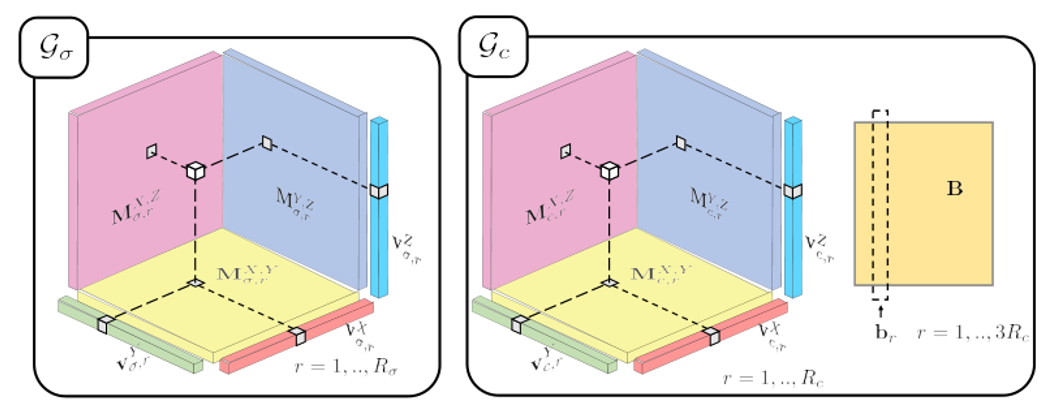
\includegraphics[width=1.0\linewidth]{fig/tensorf_vm.png}
  \caption{TensoRF中基于VM分解辐射场建模表示。注意到,每个原始网格中的体素对应着VM分解中的一个XYZ模式上的向量或矩阵因子。右侧的矩阵代表将若干$\bold b_r$向量拼接而成的全局矩阵$\bold B$。}
  \label{fig:tensorf}
\end{figure}

基于因子分解的模型可以低成本计算每个体素的特征向量,每个XYZ模式向量/矩阵因子只需要一个值即可进行估计。对张量进行三线性插值则可以构建更为精细的连续场从而提高重建质量。根据该建模得到的辐射场表示为:
\begin{equation}
  \sigma, c=\sum_{r} \sum_{m} \mathcal{A}_{\sigma, r}^{m}(\mathbf{x}), S\left(\mathbf{B}\left(\oplus\left[\mathcal{A}_{c, r}^{m}(\mathbf{x})\right]_{m, r}\right), d\right)
\end{equation}
\label{eq:10}
其中$\oplus$可以看作是将所有标量值(1通道向量)连接为$3R_c$通道向量的连接运算符。实践中需要并行计算大量体素的时候,只需要首先计算并拼接所有体素,按列向量生成一个矩阵$\mathcal A^m_{c,r,ijk}$,然后直接与$\bold B$做矩阵乘法即可。在给定任何3D位置和观看方向的情况下,都可以获得连续的体积密度和与观测方向相关的颜色。这允许高质量的辐射场重建和渲染。

在训练中,除了真实颜色与预测颜色的误差损失外,为了鼓励张量因子参数的稀疏性,还应用了标准的L1正则化,从而有效地提高外推视图的质量,并在最终渲染中去除噪点。对于输入图像很少或捕获条件不完美的真实数据集,加入了TV损失以加强监督。

\subsection{基于HY分解的张量辐射场}

VM分解由于将二者成分进行了耦合,因此实际比例是固定的。HY分解相较于VM分解,更易于灵活控制向量分量和矩阵分量的比例,这也增加了对于辐射场建模的灵活性以及可压缩、可组合性。

为了减少MLP参数过大对于模型的影响以及分解紧凑型的损失,可以使用球谐函数对5-DoF输入中的观测方向进行拟合建模。具体来说,对于一个有最大degree为$\ell_{\max}$ 的球谐函数,需要$(\ell_{\max}+1)^2$ 个球谐系数来对每个通道的颜色进行建模。对于这些系数,也可以用张量来进行表示:
\begin{equation}
  \ell_{\max }\mathcal{T}_{i, j, k}^{\kappa} \in \mathbb{R}^{\left(\ell_{\max }+1\right)^{2}}, \kappa \in\{r, g, b\}
\end{equation}
\label{eq:11}
每个位置的密度和颜色可以通过以下公式得到:
\begin{equation}
  \sigma=\phi\left(\mathcal{T}^{\text {density }}\right) \\ c^{\kappa}=\psi\left(\sum_{\ell=0}^{\ell_{\max }} \sum_{m=-\ell}^{\ell} \mathcal{T}_{\ell, m}^{\kappa} Y_{\ell}^{m}(\mathbf{d})\right), \kappa \in\{r, g, b\}
\end{equation}
\label{eq:12}
其中$\phi(\cdot),\psi(\cdot)$ 都是激活函数,$\bold d$ 是观测方向,$Y^m_{\ell}$ 是球谐函数基。通过以上方式,可以在可微渲染的过程中进行分解模式的学习。

除此之外,基于HY分解的张量辐射场还可以通过分解成分的秩的残差来进行场景压缩与组合。参考SVD分解的原理,秩越低,分解约紧凑,成分所表达的信息越重要。这也是诸如PCA等降维方法的重要原理。假设总共的分解得到$R$个秩,训练阶段数量为$M$,可以将所有的秩成分按序列分到$M$个组当中,记每个组的秩数量为$R_m$,$m\in\{1,2,...,M\}$。在训练过程中,每一次收敛后对秩成分进行固定并附加下一个秩残差项$R_m-R_{m-1}$。通过对秩残差损失的监督,我们可以更快学习到每一个组分对于基本组分的补充信息,从而在很小的模型容量的情况下获得很高的视觉质量。在实践中,这对于LOD(Level-of-Details)的设置有着很重要的效果,能够根据场景的复杂程度以及重要程度进行高保真压缩。

\section{总结与展望}
\label{sec:conclusion}


%%%%%%%%% REFERENCES
{\small
\bibliographystyle{ieee_fullname}
\bibliography{egbib}
}

\end{document}
